\chapter{Whole-Part}

\section{Summary}
Das Whole-Part Design Pattern hilft bei Zusammenführung von Komponenten zu einer logischen Einheit. Dabei wird die ganze Einheit als \textit{Whole} bezeichnet und die einzelnen Teile als \textit{Part}. Das Whole koordiniert die Zusammenarbeit der Parts und bietet ein Interface für alles. Direkter Zugriff auf die Parts ist nicht möglich.
\section{Context}
Implementierung von zusammengesetzten Objekten.
\section{Problem}
Gegeben ist ein komplexes Objekt. Nun soll dieses entweder in kleinere Teilobjekte zerteilt, oder aus weiteren Objekten zu einem ganzen verbunden werden. Clients sollten das Objekt als eine Einheit sehen, welche keinen direkten Zugriff auf die Einzelteile bietet.
\section{Solution}
Es wird mittels des Whole-Part Pattern eine Komponente eingeführt welche die kleineren Objekte in sich kapselt. Diese Komponente definiert ausserdem ein Interface für den Zugriff auf seine Funktionen, und verhindert den direkten Zugriff auf die Einzelteile.  \\
Die Beziehung zwischen Whole und Part kann drei verschiedene Ausprägungen haben:
\begin{enumerate}
	\item \textit{assembly-parts:} Alle Teile sind Eng integriert. Die Anzahl und Art der Teile ist vordefiniert und ändert sich nicht.
	\item \textit{container-contents:} Die Teile sind nicht so Eng gekuppelt wie beim assembly-parts. Es können dynamisch Teile hinzugefügt oder entfernt werden.
	\item \textit{collection-members:} Die Collection gruppiert ähnliche Teile. Es wird kein Unterschied zwischen den einzelnen Teilen gemacht, alle werden gleich behandelt.
\end{enumerate}
\subsection{Structure}
Beim Whole-Part Pattern gibt es zwei Arten von Teilnehmern.
Ein \textit{Whole} Objekt repäsentiert eine Sammlung kleinerer Objekte, welche man  \textit{Part} nennt. Über ein Interface bietet ein Whole eigene Funktionen, sowie die einzelner Parts an. Die folgende Grafik illustriert dieses Zusammenspiel nochmals:
\begin{figure}[H]
	\centering
	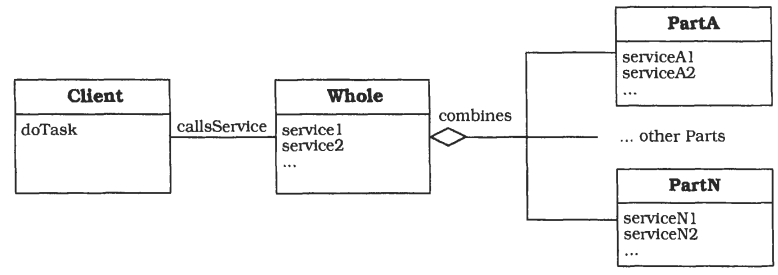
\includegraphics[width=0.7\textwidth]{figures/07-wholepart-1}
	\caption{Whole-Part Zusammenspiel}
\end{figure}
Diese Beziehungen orientieren sich an Beziehungen in der echten Welt und lassen sich manchmal auch nicht so genau abgrenzen. 
Wichtig dabei ist, dass die Kategorien die Beziehungen zwischen Objekten und nicht zwischen Datentypen beschreiben.

\section{Consequences}
\begin{itemize}
    \pro{\textbf{Änderbarkeit von Parts:} Interne Struktur kann geändert werden, da Client nur äusseres Whole sieht.}
    \pro{\textbf{Separation of concerns:} Jeder concern ist von einem separaten Part implementiert. }
    \pro{\textbf{Wiederverwendbarkeit:} Teile eines Whole können zu anderen Wholes zusammengesetzt werden.}
    \con{\textbf{Geringere Effizienz durch Indirektion:} Da ein Whole einen Wrapper um die Parts bilded, gibt es eine Ebene Indirektion mehr zwischen Client und Part. Dies kann zu Runtime Overhead führen.}
    \con{\textbf{Komplexität von Dekomposition in Parts:} Kann u.U. schwer sein, die richtige Trennung zu finden.}
\end{itemize}

\section{Known Uses}
\begin{itemize}
	\item Viele objektorientierte Applikation sind nach dem Whole Part pattern aufgebaut, oft nach dem Composite pattern
	\item Die meisten objektorientierten Klassen Libraries bieten Listen, Sets und Maps. Diese implementieren die Collection-Member und Container-Contents Varianten.
	\item Toolkits für grafische User Interfaces wie Fresco oder ET++ arbeiten nach der Composite Variante. 
\end{itemize}

\section{Relationships}
\begin{itemize}
	\item \textit{Shared Parts:} Mehrere Whole Objekte können sich einzelne Parts teilen. Lifetime von Part ist nicht mehr an Whole gebunden. Bsp: Mail mit Anhang, Anhang kann einem neuen Mail angehängt werden und bleibt bestehen, wenn erstesMail gelöscht.
	\item \textit{Assembly Parts:} In dieser Variante ist das Whole ein Objekt, welches aus kleineren Objekten besteht (z.B. ein Auto besteht aus Rädern, Motor, etc.) Dabei kann auch Rekursion entstehen, denn das Rad wiederum besteht z.B. aus Felge und Reifen.
	\item \textit{Container-Contents:} In dieser Variante ist das Whole Objekt für die Verwaltung von unterschiedlichen Inhalten verantwortlich. Im Unterschied zu der Assembly-Parts Variante können Komponenten dynamisch hinzugefügt oder entfernt werden.
	\item \textit{Collection-Members:} Diese Variante ist eine Spezialisierung des Container-Contents, bei dem alle Part-Objekte vom gleichen Typ sind.
	\item \textit{Composite pattern:} Dieses Pattern ist anwendbar für Whole-Part-Hierarchien, bei denen sowohl Whole als auch Part das selbe abstrakte Interface implementieren.
\end{itemize}

\section{Exam Questions}
\begin{itemize}
  	\item Behauptung: dies ist eine Behauptung? (Lösung)
    \item Frage: Dies ist eine Frage? (Lösung)
\end{itemize}
